\section{Methods}
As shown in Table~\ref{tab:comparison}, existing methods either keep graph exploration fixed, retrieve only once, or train on question--answer data written by humans or closed-source models with fixed difficulty. EoG (Figure~\ref{fig:framework}) consists of Graph Self-Play (Section~\ref{sec:selfplay}), SVTS (Section~\ref{sec:svts}), and the Boundary-Aware Graph Curriculum (Section~\ref{sec:frontier}), which address challenges (1)--(3) of Section~\ref{sec:intro}, respectively.

\begin{figure*}[t!]
    \centering
    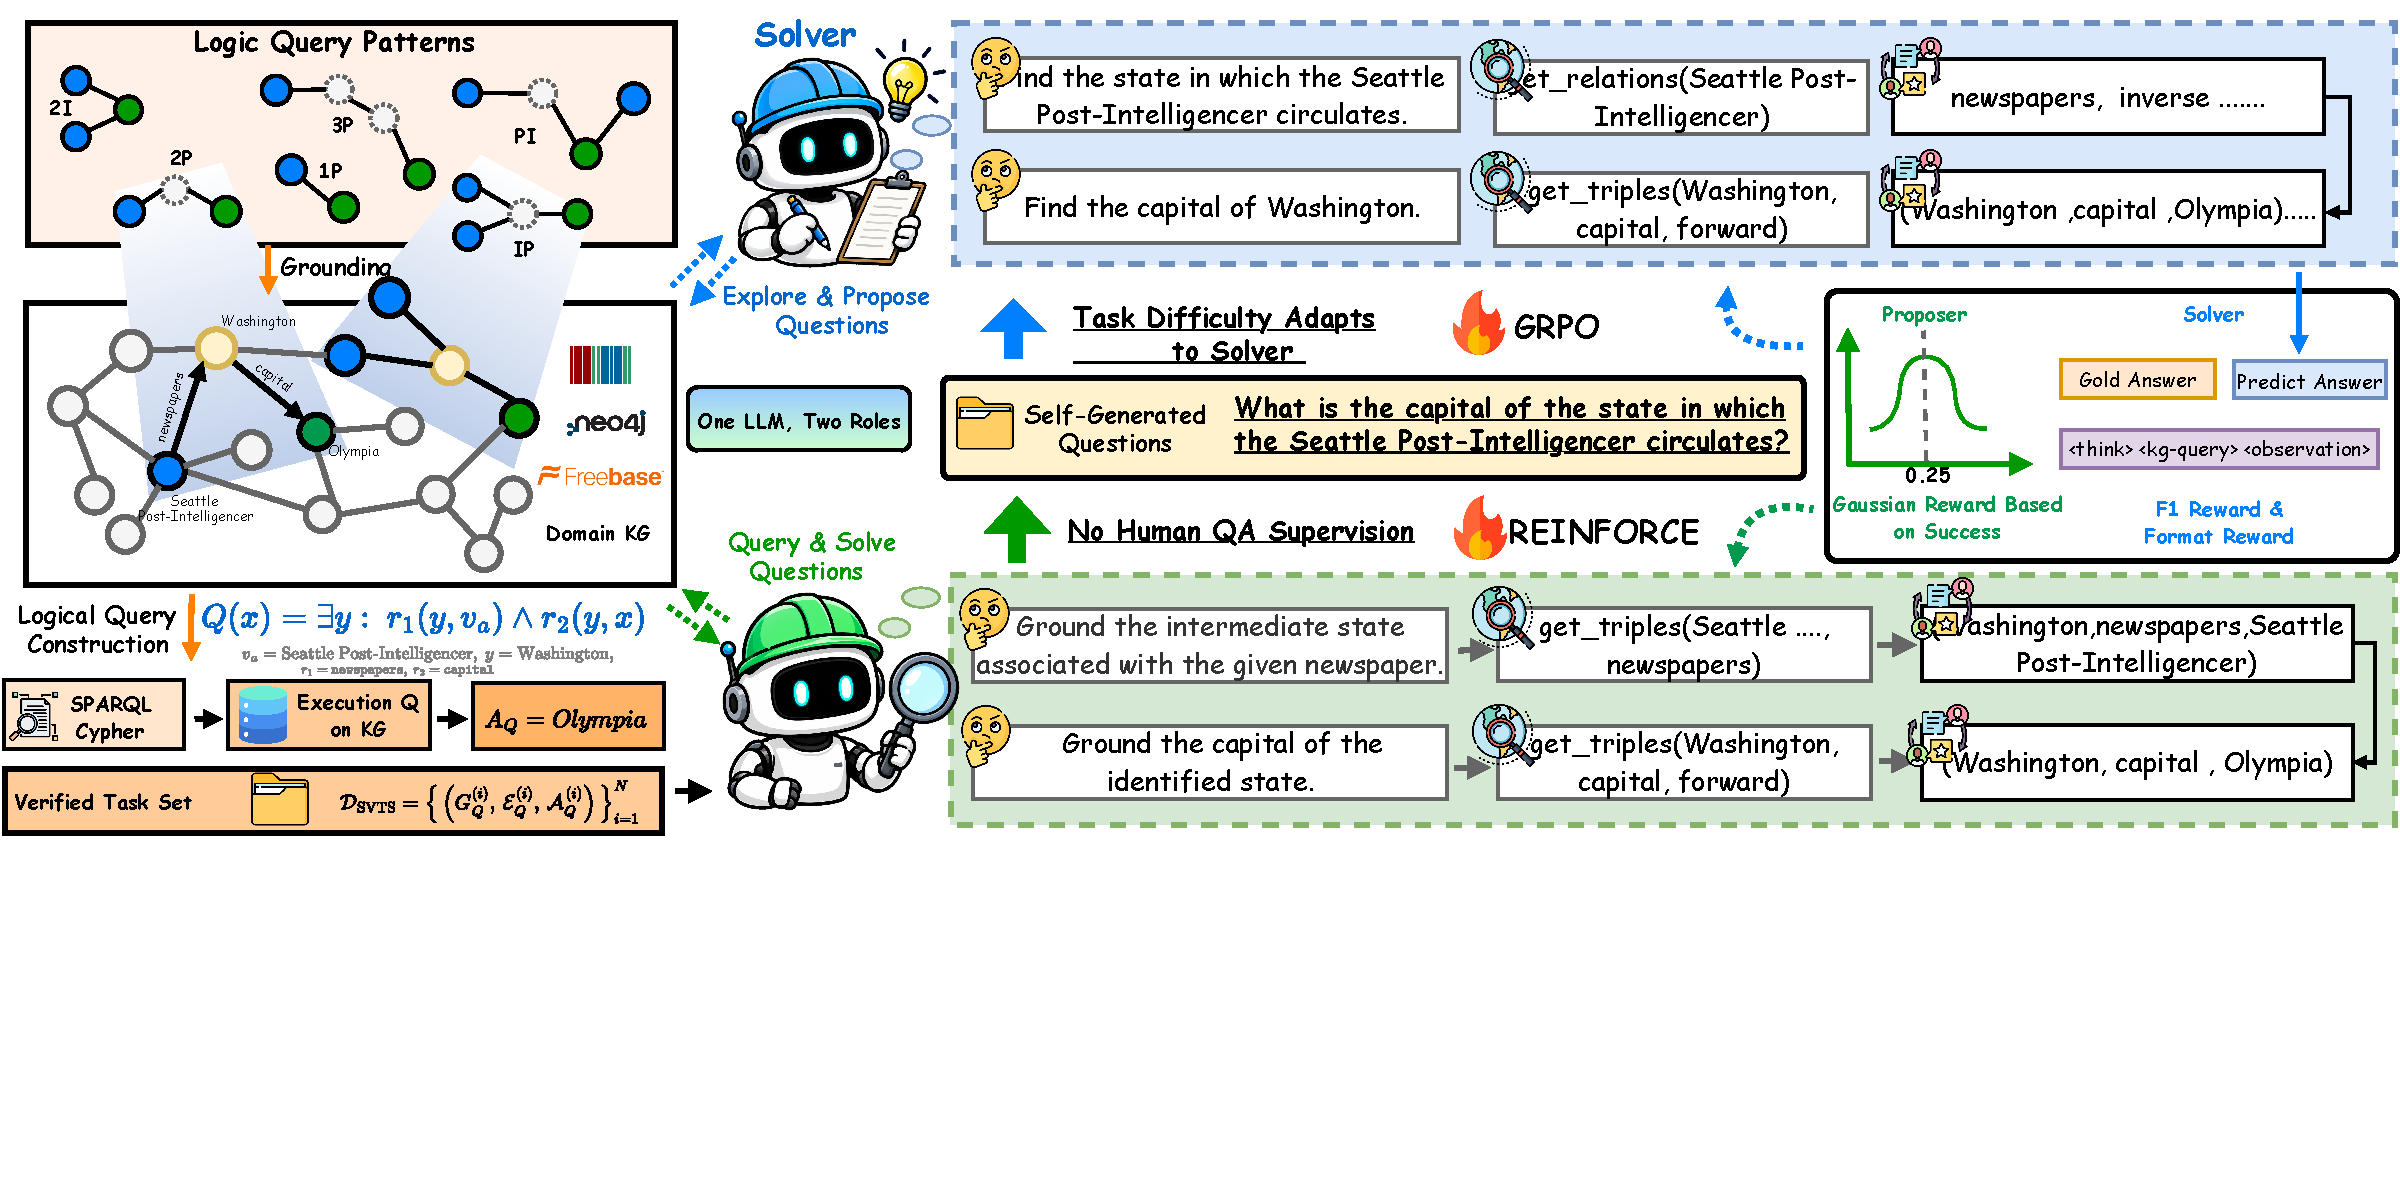
\includegraphics[width=\textwidth]{figures/main_methods.pdf}
    \caption{\textbf{Overview of EoG.} One LLM self-plays as the Proposer and the Solver, synthesizes verifiable tasks with SVTS, and forms a boundary-aware curriculum by rewarding the Proposer for questions on the Solver's capability boundary.}
    \label{fig:framework}
\end{figure*}
\subsection{Problem Formulation}
\label{sec:formulation}

\textbf{Definition 1: Logic Query.}
A knowledge graph $\mathcal{G}=(\mathcal{E},\mathcal{R},\mathcal{T})$ has an entity set $\mathcal{E}$, a relation set $\mathcal{R}$, and a triple set $\mathcal{T}\subseteq\mathcal{E}\times\mathcal{R}\times\mathcal{E}$. A multi-hop question corresponds to a first-order logic query
\begin{equation}
\label{eq:query}
\phi(x)=\exists\,y_1,\ldots,y_k:\ e_1\wedge e_2\wedge\cdots\wedge e_n,
\end{equation}
where $x$ is the answer variable, $y_1,\ldots,y_k$ are intermediate variables, and each atom $e_i=r(u,u')$ links an anchor entity or a variable to a variable and is true if and only if $(u,r,u')\in\mathcal{T}$. The answer set of $\phi$ is its denotation $\llbracket\phi\rrbracket_{\mathcal{G}}=\{a\in\mathcal{E}\mid\phi(a)=\mathrm{True}\}$.

\textbf{Definition 2: Graph Environment.}
Following GraphWalker~\citep{GraphWalker}, an agent interacts with $\mathcal{G}$ in a think--query--observe loop through two tools: \texttt{get\_relations} returns the relations of an entity, and \texttt{get\_triples} returns its triples under given relations. At step $t$, given the state $s_t$ of all previous turns, the agent takes an action $a_t$, a tool call or a final answer, and observes triples $o_t\subseteq\mathcal{T}$. A trajectory $\tau=(a_1,o_1,\ldots,a_T)$ collects the evidence
\begin{equation}
\label{eq:evidence}
\mathcal{O}(\tau)=\textstyle\bigcup_{t=1}^{T}o_t\subseteq\mathcal{T},
\end{equation}
where the last action $a_T$ gives the final answer $\mathcal{A}(\tau)\subseteq\mathcal{E}$.

\textbf{Problem Statement.}
Given $\mathcal{G}$ and an initial policy $\pi_{\theta_0}$, we learn a policy $\pi_\theta$ that maximizes the expected F1 of answering multi-hop questions on $\mathcal{G}$, without any question--answer pair or closed-source model. Training uses only symbolic tasks $d=(G_Q,\mathcal{E}_Q,\mathcal{A}_Q)$ built from $\mathcal{G}$, where the query graph $G_Q$ grounds a query $\phi$ on $\mathcal{G}$, $\mathcal{E}_Q$ is its set of anchor entities, and $\mathcal{A}_Q=\llbracket\phi\rrbracket_{\mathcal{G}}$ is its gold answer set.

\subsection{Graph Self-Play}
\label{sec:selfplay}

To let the exploration ability improve through interaction, we propose Graph Self-Play, in which a single policy $\pi_\theta$ plays two roles under different role prompts with shared parameters: the Proposer $\pi_\theta^{\mathrm{P}}$ turns a task into a natural-language question, and the Solver $\pi_\theta^{\mathrm{S}}$ answers it. Both roles reason inside \texttt{<think>}, call the graph tools of Definition~2 inside \texttt{<kg-query>}, and read the returned triples inside \texttt{<information>} blocks, so both act by exploring the same graph. The Solver aims to answer correctly, while the Proposer aims to pose valid questions that the Solver can learn from:
\begin{equation}
\label{eq:game}
\begin{aligned}
&\max_{\pi_\theta^{\mathrm{S}}}\ \mathbb{E}_{d,\;q\sim\pi_\theta^{\mathrm{P}},\;\rho\sim\pi_\theta^{\mathrm{S}}}\bigl[R_{\mathrm{S}}(\rho)\bigr],\\
&\max_{\pi_\theta^{\mathrm{P}}}\ \mathbb{E}_{d,\;q\sim\pi_\theta^{\mathrm{P}}}\bigl[R_{\mathrm{P}}(q)\bigr]\quad\text{s.t.}\quad v(q)=1,
\end{aligned}
\end{equation}
where $d$ is a task synthesized by SVTS, $R_{\mathrm{S}}$ is the Solver reward defined below, $v(q)$ is the validity check of Section~\ref{sec:svts}, and $R_{\mathrm{P}}$ of Section~\ref{sec:frontier} depends on the Solver's performance on $q$. Since the two roles share $\theta$, the policy gains exploration experience both when it poses a question and when it searches for the answers. It includes question generation, question solving, and Solver optimization.

\paragraph{Question generation.}
For each task $d=(G_Q,\mathcal{E}_Q,\mathcal{A}_Q)$, the Proposer reads the reasoning skeleton of $G_Q$, in which only the anchors appear as real entity names, while the intermediate and answer entities appear as placeholders. For example, the skeleton Goodison Park $\xleftarrow{\texttt{arena\_stadium}}$ \texttt{Mid1@} $\xrightarrow{\texttt{owner\_s}}$ \texttt{Ans@} should become ``Who is the owner of the team that plays at Goodison Park?''. Since the tools cannot be called on placeholders, the Proposer explores the graph over multiple turns from the real anchors $\mathcal{E}_Q$ to uncover the facts, and produces a trajectory $\tau^{\mathrm{P}}$ that ends with a question
\begin{equation}
\label{eq:propose}
q\sim\pi_\theta^{\mathrm{P}}(\cdot\mid G_Q,\mathcal{E}_Q,\mathcal{G}),
\end{equation}
where $q$ is extracted from the final \texttt{<result>} block of $\tau^{\mathrm{P}}$. The prompt asks $q$ to name the anchors, keep the full reasoning chain of the skeleton, and hide intermediate and answer entities, so that answering $q$ needs the same multi-hop reasoning as the task.

\paragraph{Question solving.}
For a question $q$, the Solver starts from the anchors $\mathcal{E}_Q$ given in its prompt and samples a group of $n$ trajectories through multi-turn interaction with the graph,
\begin{equation}
\label{eq:solve}
\rho^{j}\sim\pi_\theta^{\mathrm{S}}(\cdot\mid q,\mathcal{E}_Q,\mathcal{G}),\qquad j=1,\ldots,n,
\end{equation}
where the Solver decides which relations and entities to explore and when to stop, and each trajectory ends with a JSON list of entity names in an \texttt{<answer>} block, which gives the prediction $\hat{y}^{j}=\mathcal{A}(\rho^{j})$. Each trajectory is scored by answer and format:
\begin{equation}
\label{eq:rs}
R_{\mathrm{S}}(\rho^{j})=\lambda_{\mathrm{ans}}\,\mathrm{F1}\bigl(\hat{y}^{j},\mathcal{A}_Q\bigr)+\lambda_{\mathrm{fmt}}\,R_{\mathrm{fmt}}(\rho^{j}),
\end{equation}
where the first term is the F1 between the predicted and gold answer sets, $R_{\mathrm{fmt}}\!\in\![0,1]$ measures how well the trajectory follows the think--query--observe structure, and the weights are $\lambda_{\mathrm{ans}}=0.8$ and $\lambda_{\mathrm{fmt}}=0.2$. We use F1 rather than exact match because a task may have several gold answers, so a prediction that recovers only part of $\mathcal{A}_Q$ still receives partial credit. Since $R_{\mathrm{S}}$ scores only the final answer, any exploration path that reaches $\mathcal{A}_Q$ is rewarded, so the Solver learns its own exploration strategy from interaction.

\paragraph{Solver optimization.}
The Solver is updated with GRPO. For a group $\{\rho^{j}\}_{j=1}^{n}$ on the same $q$, the relative advantage is $\hat{A}^{j}=\bigl(R_{\mathrm{S}}(\rho^{j})-\mathrm{mean}\bigr)/\mathrm{std}$, with $\mathrm{mean},\mathrm{std}$ over $\{R_{\mathrm{S}}(\rho^{k})\}_{k=1}^{n}$, and the objective is
\begin{equation}
\label{eq:grpo}
\begin{aligned}
\mathcal{J}_{\mathrm{S}}(\theta)
=\mathbb{E}\!\Bigg[\frac1n\sum_{j=1}^{n}\frac{1}{|\rho^{j}|}
\sum_{t=1}^{|\rho^{j}|}
\min\!\Big(&w^{j}_{t}\hat{A}^{j},
&\operatorname{clip}(w^{j}_{t},1-\epsilon,1+\epsilon)\hat{A}^{j}\Big)\Bigg]\\
-\beta\,\mathbb{D}_{\mathrm{KL}}\!\left[\pi_\theta^{\mathrm{S}}\,\|\,\pi_{\mathrm{ref}}\right],
\end{aligned}
\end{equation}
where $w^{j}_{t}=\pi_\theta^{\mathrm{S}}\bigl(a^{j}_{t}\mid s^{j}_{t}\bigr)/\pi_{\theta_{\mathrm{old}}}^{\mathrm{S}}\bigl(a^{j}_{t}\mid s^{j}_{t}\bigr)$ is the token-level importance ratio at step $t$, $\epsilon$ is the clipping threshold, and $\beta$ is the KL coefficient.

\subsection{Symbolically Verifiable Topology Synthesis}
\label{sec:svts}

To obtain reliable training data without human annotation or closed-source models, we propose SVTS, which views the KG as a first-order logic structure and takes query execution on the graph as the source of gold answers. It includes three steps: defining query patterns, grounding and execution, and question verification.

\paragraph{Query patterns.}
Following complex logical queries over KGs~\citep{ren2020betae}, we define six query patterns as reasoning topologies:
\begin{equation}
\mathcal{P}=\{1p,\,2p,\,3p,\,2i,\,ip,\,pi\},
\end{equation}
where $p$ and $i$ denote projection (one hop along a relation) and intersection (multiple constraints on one variable), respectively; $1p$--$3p$ are $1$- to $3$-hop chain queries, $2i$ is a two-way intersection, and $ip$, $pi$ are nested compositions of projection and intersection. For example, the $2p$ and $2i$ query patterns are written as
\begin{equation}
\label{eq:2p-2i}
\begin{aligned}
\phi_{2p}(x)&=\exists y:\ r_1(v_a,y)\wedge r_2(y,x),\\
\phi_{2i}(x)&=r_1(v_{a_1},x)\wedge r_2(v_{a_2},x),
\end{aligned}
\end{equation}
where $\phi_{2p}$ follows a two-hop chain from one anchor, whereas $\phi_{2i}$ requires the answer to satisfy constraints from two anchors; the logical forms of all six patterns are listed in Appendix~\ref{app:algorithm}. On Freebase, the synthesized questions cover all six patterns, with shares ranging from $9.5\%$ ($pi$) to $22.4\%$ ($1p$), so the Solver must learn path expansion, constraint intersection, and intermediate-variable tracking rather than fit a single pattern (Appendix~\ref{app:contamination}).

\paragraph{Grounding and execution.}
Given a pattern $pat\in\mathcal{P}$, grounding instantiates $pat$ on real facts and extracts its grounded query graphs $\mathcal{I}_{pat}=f_{pat}(\mathcal{G})$, where $f_{pat}$ is the corresponding extraction procedure: it samples a seed entity from a seed pool and walks on $\mathcal{G}$ to bind every variable and relation of $pat$ to a real triple, and it repeats until a target number of tasks per pattern is collected or an attempt budget runs out. The walk only proposes the structure of a task; its answers are decided by execution below. For example, a $2p$ grounded query graph sampled from Freebase is Shaping~$\xrightarrow{\texttt{recipes}}$ Country Sourdough Bread~$\xrightarrow{\texttt{techniques}}$~$x$, whose execution returns two answers, Kneading and Slashing~dough. We then compile each $G_Q\in\mathcal{I}_{pat}$ deterministically into an executable KG query $Q$ for the logic query $\phi$ of Equation~\ref{eq:query}, and evaluate it on $\mathcal{G}$ to obtain the complete gold answer set, i.e., the denotation of $\phi$:
\begin{equation}
\label{eq:exec-main}
\mathcal{A}_Q=\mathrm{Execute}(Q,\mathcal{G})=\llbracket\phi\rrbracket_{\mathcal{G}},
\end{equation}
where queries whose answers are empty, abnormally large, or unnameable are discarded rather than truncated, so that every kept task has an answer set that can be checked objectively. Unlike random-walk synthesis, which takes a single entity of the walk as the answer, execution returns every entity that satisfies the query. This entity is always one of these answers, but when $|\mathcal{A}_Q|>1$, scoring a complete prediction against it alone would give an F1 of only $2/(1+|\mathcal{A}_Q|)$. SVTS runs once per KG before training and only needs query access to the KG, so applying EoG to a new KG requires only its query endpoint. It finally outputs the task set
\begin{equation}
\label{eq:dsvts}
\mathcal{D}_{\mathrm{SVTS}}=\bigl\{(G_Q^{(i)},\mathcal{E}_Q^{(i)},\mathcal{A}_Q^{(i)})\bigr\}_{i=1}^{N},
\end{equation}
where $N$ is the task count (Algorithm~\ref{alg:svts} in Appendix~\ref{app:algorithm}).

\paragraph{Question verification.}
Execution guarantees that $\mathcal{A}_Q$ answers the query $Q$, but not that the question $q$ written by the Proposer expresses the same query. To keep $q$ faithful to its task, we collect the evidence $\mathcal{O}(\tau^{\mathrm{P}})$ retrieved by the Proposer and let the Solver answer $q$ using \emph{only} that evidence as a verifier:
\begin{equation}
\label{eq:verify}
\sigma\sim\pi_\theta^{\mathrm{S}}\bigl(\cdot\mid q,\mathcal{E}_Q,\mathcal{O}(\tau^{\mathrm{P}})\bigr).
\end{equation}
A question is valid only if it passes a rule check $v_{\mathrm{rule}}(q)$, which requires that $q$ can be extracted from the \texttt{<result>} block, has a reasonable length, and names no intermediate or answer entity, and if the verification answer matches the gold answer:
\begin{equation}
\label{eq:valid}
v(q)=v_{\mathrm{rule}}(q)\cdot\mathbb{I}\bigl[\,\mathcal{A}(\sigma)=\mathcal{A}_Q\,\bigr]\in\{0,1\},
\end{equation}
where $\mathbb{I}[\cdot]$ is the indicator function. Only questions with $v(q)=1$ enter reward computation and policy update. The rule check removes questions that leak intermediate or answer entities. The evidence check removes questions that are ambiguous, under-specified, or inconsistent with their task: since the verifier sees only the Proposer's triples, it recovers exactly $\mathcal{A}_Q$ only if these triples, read through $q$, determine the complete answer set. The check is conservative: a faithful question may be rejected when the single verification trajectory $\sigma$ fails, lowering the yield of valid questions, but a question whose evidence does not determine $\mathcal{A}_Q$ is never accepted.

\subsection{Boundary-Aware Graph Curriculum}
\label{sec:frontier}

To let task topologies follow the Solver's ability, we propose the Boundary-Aware Graph Curriculum, which rewards the Proposer by the Solver's score variance, so that it keeps posing questions on the Solver's capability boundary. It includes three parts: the capability boundary, the Proposer reward, and Proposer optimization.

\paragraph{Capability boundary.}
For a valid question $q$ with Solver trajectories $\{\rho^{j}\}_{j=1}^{n}$, let $s_j=\mathrm{F1}(\hat{y}^{j},\mathcal{A}_Q)\in[0,1]$ be the answer score of $\rho^{j}$ in Equation~\ref{eq:rs} and $\bar{s}(q)$ their mean. The Solver's score variance on $q$, which measures how differently its trajectories score, is
\begin{equation}
\label{eq:cbar}
\sigma^{2}(q)=\frac1n\sum_{j=1}^{n}\bigl(s_j-\bar{s}(q)\bigr)^{2}.
\end{equation}
Since the advantages in Equation~\ref{eq:grpo} are normalized within a group, a question on which all $n$ trajectories receive the same score ($\sigma^{2}(q)=0$), such as one the Solver always or never solves, gives almost no learning signal~\citep{DAPO}. The Solver learns mainly from questions with $\sigma^{2}(q)>0$, which it has not mastered but can still partly solve, such as one it answers in full on some trajectories and only in part on others; we call them its \emph{capability boundary}.

\paragraph{Proposer reward.}
We therefore reward the Proposer with a Gaussian boundary reward on the Solver's score variance:
\begin{equation}
\label{eq:rp}
R_{\mathrm{P}}(q)=\exp\!\left(-\frac{\bigl(\sigma^{2}(q)-\tfrac14\bigr)^{2}}{2h}\right),
\end{equation}
where $h>0$ controls the peak width. Since scores lie in $[0,1]$, $\sigma^{2}(q)\le\tfrac14$, with equality only when half of the trajectories score $1$ and the rest $0$. The reward is thus minimal, $\exp(-\tfrac{1}{32h})$, when all scores are equal, higher on the capability boundary, and maximal at such an even split. As the scores are F1 against the complete answer sets of SVTS, a question the Solver answers only in part stays on the boundary instead of counting as solved. The reward also stays low when every trajectory fails, so the Proposer is not reinforced by questions the Solver cannot learn from.

\textbf{Proposition 1.} \textit{With equal format scores, $R_{\mathrm{P}}$ is maximal only where the learning signal peaks and minimal where it vanishes.}\vspace{-2mm}
\begin{proof}
We provide experimental results on the Proposer rewards in Section~\ref{sec:rq-frontier} and a proof in Appendix~\ref{app:proof}.
\end{proof}

\begin{table*}[t!]
    \caption{\textbf{Main results on five public KGQA benchmarks} (Hit@1 and F1, \%; IndustryCarBench in Figure~\ref{fig:carbench}). Full-supervised methods are for reference, with icons marking training sets; bold marks the best annotation-free result; ``--'' means not evaluated.}
    \centering
    \footnotesize
    \setlength{\tabcolsep}{4pt}
    \renewcommand{\arraystretch}{1.05}

    \resizebox{\textwidth}{!}{
    \begin{tabular}{ll*{12}{c}}
        \toprule
        \multirow{2}{*}{\textbf{Method}} & \multirow{2}{*}{\textbf{LLM}}
        & \multicolumn{2}{c}{\textbf{WebQSP}~\icW}
        & \multicolumn{2}{c}{\textbf{CWQ}~\icC}
        & \multicolumn{2}{c}{\textbf{GrailQA}~\icG}
        & \multicolumn{2}{c}{\textbf{GTSQA}~\icT}
        & \multicolumn{2}{c}{\textbf{WikiWebQuestions}}
        & \multicolumn{2}{c}{\textbf{Avg.}} \\
        \cmidrule(lr){3-4} \cmidrule(lr){5-6} \cmidrule(lr){7-8} \cmidrule(lr){9-10} \cmidrule(lr){11-12} \cmidrule(lr){13-14}
        & & \textbf{Hit@1} & \textbf{F1} & \textbf{Hit@1} & \textbf{F1} & \textbf{Hit@1} & \textbf{F1}
        & \textbf{Hit@1} & \textbf{F1} & \textbf{Hit@1} & \textbf{F1} & \textbf{Hit@1} & \textbf{F1} \\
        \midrule
        \rowcolor{gray!15}
        \multicolumn{14}{c}{\textit{Full-Supervised Methods}} \\
        \midrule
        \rowcolor{rlbg}
        KG-R1$^\dagger$~\icW & Qwen-2.5-7B & 78.42 & 69.02 & 50.92 & 46.88 & 61.64 & 59.29 & -- & -- & -- & -- & 63.66 & 58.40 \\
        \rowcolor{rlbg}
        KG-R1$^\dagger$~\icC & Qwen-2.5-7B & 80.71 & 68.57 & 58.03 & 53.93 & 67.81 & 65.52 & -- & -- & -- & -- & 68.85 & 62.67 \\
        \rowcolor{rlbg}
        KG-R1$^\dagger$~\icG & Qwen-2.5-7B & 71.06 & 61.64 & 46.02 & 42.43 & 69.13 & 64.88 & -- & -- & -- & -- & 62.07 & 56.32 \\
        \rowcolor{rlbg}
        KG-R1$^\dagger$~\icT & Qwen-2.5-7B & -- & -- & -- & -- & -- & -- & 48.03 & 49.23 & 75.39 & 66.28 & 61.71 & 57.76 \\
        \midrule
        \rowcolor{gray!15}
        \multicolumn{14}{c}{\textit{Annotation-Free Methods}} \\
        \midrule
        \rowcolor{promptbg}
        & Qwen-2.5-3B & 32.21 & 20.60 & 12.42 & 13.72 & 11.00 & 8.70 & 7.83 & 7.45 & 37.43 & 23.00 & 20.18 & 14.69 \\
        \rowcolor{promptbg}
        & Qwen-2.5-7B & 38.50 & 24.20 & 24.61 & 20.25 & 11.70 & 8.96 & 10.11 & 9.16 & 45.87 & 28.45 & 26.16 & 18.20 \\
        \rowcolor{promptbg} \multirow{-3}{*}{IO} & LLaMA-3.1-8B & 48.14 & 31.79 & 29.85 & 24.30 & 16.30 & 11.13 & 12.95 & 11.56 & 51.99 & 34.09 & 31.85 & 22.57 \\
        \midrule
        \rowcolor{promptbg}
        & Qwen-2.5-3B & 34.96 & 22.20 & 17.76 & 15.00 & 11.00 & 8.70 & 5.73 & 4.92 & 39.83 & 23.41 & 21.86 & 14.85 \\
        \rowcolor{promptbg}
        & Qwen-2.5-7B & 40.94 & 26.98 & 28.38 & 23.70 & 15.40 & 12.25 & 10.23 & 9.15 & 47.30 & 30.27 & 28.45 & 20.47 \\
        \rowcolor{promptbg} \multirow{-3}{*}{CoT~\citep{CoT}} & LLaMA-3.1-8B & 43.99 & 30.01 & 23.93 & 20.18 & 15.20 & 11.16 & 9.06 & 8.27 & 51.86 & 33.87 & 28.81 & 20.70 \\
        \midrule
        \rowcolor{promptbg}
        & Qwen-2.5-3B & 50.64 & 23.50 & 29.31 & 14.99 & 22.10 & 9.81 & 13.13 & 6.40 & 40.50 & 25.47 & 31.14 & 16.03 \\
        \rowcolor{promptbg}
        & Qwen-2.5-7B & 50.58 & 27.94 & 38.97 & 26.08 & 23.00 & 12.67 & 17.76 & 9.90 & 60.46 & 31.19 & 38.15 & 21.56 \\
        \rowcolor{promptbg} \multirow{-3}{*}{SC~\citep{Self-Consistency}} & LLaMA-3.1-8B & 61.81 & 33.77 & 43.39 & 25.78 & 28.00 & 13.80 & 20.84 & 11.85 & 66.71 & 35.70 & 44.15 & 24.18 \\
        \midrule
        \rowcolor{agentbg}
        & Qwen-2.5-3B & 22.63 & 18.25 & 12.06 & 10.63 & 21.26 & 18.61 & 15.47 & 14.72 & 36.46 & 29.56 & 21.58 & 18.35 \\
        \rowcolor{agentbg}
        & Qwen-2.5-7B & 34.82 & 28.42 & 16.06 & 13.45 & 49.19 & 50.07 & 29.41 & 26.52 & 49.14 & 39.63 & 35.72 & 31.62 \\
        \rowcolor{agentbg} \multirow{-3}{*}{ReAct~\citep{React}} & LLaMA-3.1-8B & 48.42 & 40.53 & 17.73 & 15.00 & 27.33 & 28.21 & 18.87 & 17.99 & 33.83 & 28.73 & 29.24 & 26.09 \\
        \midrule
        \rowcolor{agentbg}
        ToG~\citep{ToG} & Qwen-2.5-7B & 55.22 & 43.25 & 36.90 & 35.70 & 62.95 & 56.07 & 38.04 & 34.21 & 64.52 & 49.07 & 51.53 & 43.66 \\
        \rowcolor{agentbg}
        PoG~\citep{PoG} & Qwen-2.5-7B & 49.23 & 36.83 & 32.82 & 28.57 & 57.39 & 50.79 & 35.02 & 32.40 & 53.26 & 40.14 & 45.54 & 37.75 \\
        \rowcolor{agentbg}
        CoR~\citep{CoR} & Qwen-2.5-7B & 63.27 & 57.62 & 23.23 & 21.32 & 58.70 & 54.01 & 26.63 & 24.48 & 66.39 & 54.00 & 47.64 & 42.29 \\
        \rowcolor{retrbg}
        Text-Based Retrieval & Qwen-2.5-7B & 59.86 & 42.78 & 31.61 & 28.78 & 53.64 & 46.60 & 37.73 & 36.44 & 67.22 & 50.00 & 50.01 & 40.92 \\
        \rowcolor{retrbg}
        Graph Reranker & Qwen-2.5-7B & 68.27 & 48.89 & 37.69 & 33.28 & 56.28 & 48.99 & 37.85 & 36.65 & 70.37 & 53.48 & 54.09 & 44.26 \\
        \midrule
        \rowcolor{lightblue}
        & Qwen-2.5-3B & 63.57 & 55.22 & 38.14 & 36.84 & 56.17 & 55.05 & 30.95 & 28.76 & 41.26 & 34.30 & 46.02 & 42.03 \\
        \rowcolor{lightblue} \multirow{-2}{*}{EoG (Qwen-2.5)} & Qwen-2.5-7B & 70.13 & \best{62.10} & \best{50.58} & \best{49.27} & \best{65.38} & \best{63.01} & \best{48.39} & \best{46.36} & \best{73.28} & 60.82 & \best{61.55} & \best{56.31} \\
        \midrule
        \rowcolor{lightblue}
        EoG (LLaMA-3.1) & LLaMA-3.1-8B & \best{71.82} & 61.51 & 50.36 & 48.25 & 63.87 & 62.59 & 36.37 & 34.67 & 70.53 & \best{62.55} & 58.59 & 53.91 \\
        \bottomrule
    \end{tabular}
    }
    \label{tab:main_result}
    \vspace{-2mm}
\end{table*}

\paragraph{Proposer optimization.}
Since the Proposer writes a single question per task, it has no group of samples for a relative advantage; we therefore update it with REINFORCE, taking the Proposer reward as the return of its whole question trajectory:
\begin{equation}
\label{eq:reinforce}
\mathcal{J}_{\mathrm{P}}(\theta)=\mathbb{E}\!\Bigg[
R_{\mathrm{P}}(q)\sum_{t=1}^{|\tau^{\mathrm{P}}|}
\log\pi_\theta^{\mathrm{P}}\!\bigl(a^{\mathrm{P}}_{t}\mid s^{\mathrm{P}}_{t}\bigr)
\Bigg],
\end{equation}
where $a^{\mathrm{P}}_{t}$ and $s^{\mathrm{P}}_{t}$ are the action and state of the Proposer at step $t$. The two roles update alternately: as the Solver masters a kind of question, its scores approach $1$, so $\sigma^{2}$ and $R_{\mathrm{P}}$ fall, driving the Proposer toward harder questions; the boundary thus moves outward and the two roles co-evolve into an adaptive curriculum.

\paragraph{Training loop.}
At each training step, the shared policy first acts as the Proposer on a batch of SVTS tasks and writes one question per task. Each question is checked by Equation~\ref{eq:valid}; questions that fail the check are skipped by both updates, and for every valid question the Solver samples $n$ trajectories on the graph, which yield both the Solver rewards $R_{\mathrm{S}}$ and, through $\sigma^{2}(q)$, the Proposer reward $R_{\mathrm{P}}$. The same parameters $\theta$ are then updated with GRPO on the Solver trajectories and with REINFORCE on the Proposer trajectories. Because both roles are updated at every step, a change in the Solver's ability is reflected in $R_{\mathrm{P}}$ at the next step, so the curriculum follows the Solver without a manually designed difficulty schedule. At test time, only the Solver is used, and it answers human-written questions with the same tools. The whole loop thus uses only the graph: tasks come from SVTS, answers from query execution, and difficulty from the Solver's own score variance on each question.
